\chapter{Datasets and running conditions}
\label{chap:prod:data}

The data used for this measurement were collected at the beginning of \runtwo\ 
of the \ac{LHC}, during a special 15-day `early measurements' period.
The number of bunches in the accelerator was gradually increased from 50 at the 
beginning to 482 bunches at the end of the period, with the number colliding at 
IP8 increasing from 36 to 397 bunches.
In addition, the minimum bunch spacing was set to \SI{50}{\nano\second}, as in 
\runone, rather than the nominal \runtwo\ spacing of \SI{25}{\nano\second}.
These steps were taken primarily for machine safety, as the \ac{LHC} began 
operating at a new centre-of-mass energy of \SI{13}{\TeV}.

The combined dataset used for the measurement corresponds to an integrated 
luminosity of
\begin{equation}
  \intlumi = \SI{\xsectotlumi}{\per\pico\barn}.
  \label{eqn:prod:xsectotlumi}
\end{equation}
The integrated luminosity measurement is performed using a beam-gas imaging 
technique~\cite{LHCb-PAPER-2014-047}.
For reference, the total integrated luminosity collected in \runone\ at \lhcb\ 
was \SI{3}{\per\femto\barn}, whilst that for the \sqrtseq{7}\ \lhcb\ open charm 
production measurement was \SI{15}{\per\nb}.
All data were taken with the \lhcb\ dipole magnet in the `down' polarity, and 
were processed via the Turbo stream data flow, as described in 
\cref{chap:intro:lhcb:detector}.
A matching set of simulated \ac{MC} events is also used in the analysis, which 
is described in \cref{chap:prod:data:mc}.
The selection of events and charm candidates, both in the trigger and offline, 
will be described in \cref{chap:prod:sel}.

\section{Simulated data samples}
\label{chap:prod:data:mc}

This analysis uses simulated samples of \DstToDzpi\ with \DzToKpi, \DpToKpipi, 
and \DspToKKpi\ decays.
The \DstToDzpi\ sample is sufficient for studying both \DstToDzpi\ and 
(untagged) \DzToKpi\ efficiencies, as the effect of the soft pion is 
parameterised in \PDzero\ \pT\ and \rapidity.
In addition, the \DspToKKpi\ sample is sufficient for studying \DspTophipi\ 
decays, given that the kaon pair is required to be within the same mass window 
as applied to the data.
For each decay mode, samples of \num{2.5} million events are generated, with an 
additional \num{1} million events generated where the signal charm hadron is 
required to have $\pT > \SI{10}{\GeVc}$.
To save computing resources, the signal decays are required to be within the 
\lhcb\ geometric acceptance after \evtgen\ has run.
This requires all charged final-state particles to have a positive $z$ 
component of their three-momentum and to satisfy
\begin{equation}
  10 < \theta < \SI{400}{\milli\radian},
  \label{eqn:prod:data:lhcb_acceptance}
\end{equation}
where $\theta$ is the polar angle.
As this cut is not \SI{100}{\percent} efficient in some \pTy\ bins, its 
efficiency must be assessed, as described in \cref{chap:prod:effs:acc}, and so 
dedicated, generator-only datasets are also produced.
These data are not processed beyond the \evtgen\ step.

In addition to the usual truth-matching procedure discussed in 
\cref{chap:intro:lhcb:simulation}, a prompt/secondary flag is computed for each 
candidate charm vertex, based on the true lifetime of each particle preceding 
it in the true decay chain.
If the lifetime of any particle in the true ancestry of the charm candidate 
exceeds a threshold of \SI{0.1}{\femto\second}, the candidate is flagged as 
secondary.\footnotemark\
In what follows, the \ac{MC} data have been filtered such that only 
truth-matched, prompt charm hadron candidates remain, unless stated otherwise.

\footnotetext{%
  The order of magnitude of the lifetimes of the ground-state charm and beauty 
  hadrons is between $0.1$ and \SI{1}{\pico\second}.
}

\section{Crossing angle correction}
\label{chap:prod:data:crossing_angle}

Due to the non-zero crossing angles of the proton beams, the \pp\ collision 
frame is boosted with respect to the laboratory frame.
As this measurement is made in bins of charm hadron transverse momentum and 
rapidity measured in the \pp\ collision rest frame, a correction is applied to 
the \pT\ and \rapidity\ measured in the laboratory frame.
Example \pT\ and \rapidity\ distributions as measured in the laboratory and 
\pp\ centre-of-mass frames are given for the simulated \DstToDzpi\ dataset in 
\cref{fig:prod:data:com_boost}.
Whenever charm hadron \pT\ or \rapidity\ are mentioned, it is the \pp\ rest 
frame quantities that are used, unless stated otherwise.

\begin{figure}%
  \begin{subfigure}[b]{0.5\textwidth}
    \centering
    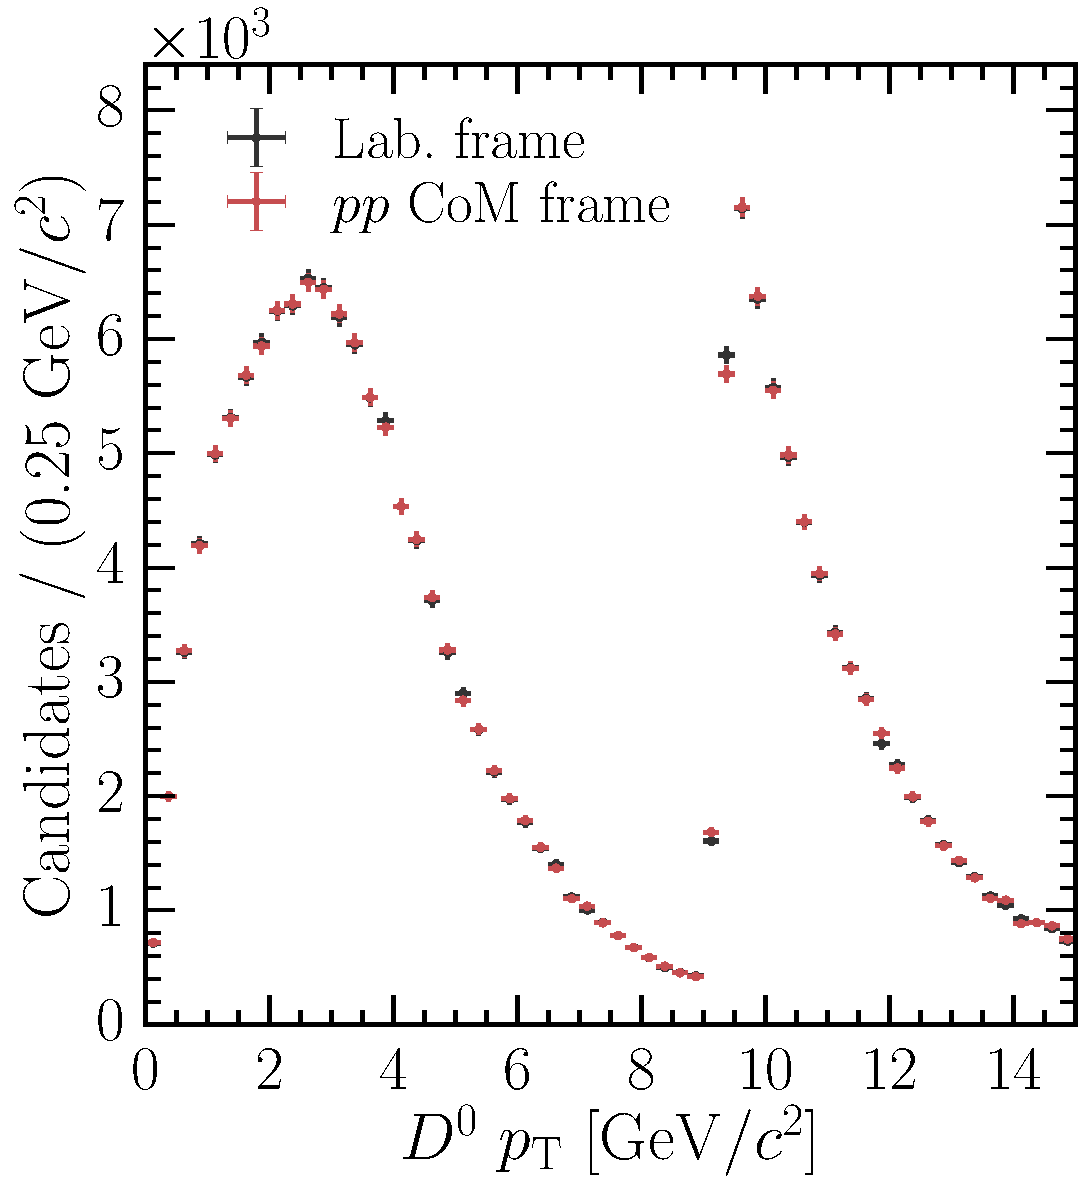
\includegraphics[width=\textwidth]{production/data/D0ToKpi_MC_PT}
    \caption{\pT}
    \label{fig:prod:data:com_boost:pt}
  \end{subfigure}
  \begin{subfigure}[b]{0.5\textwidth}
    \centering
    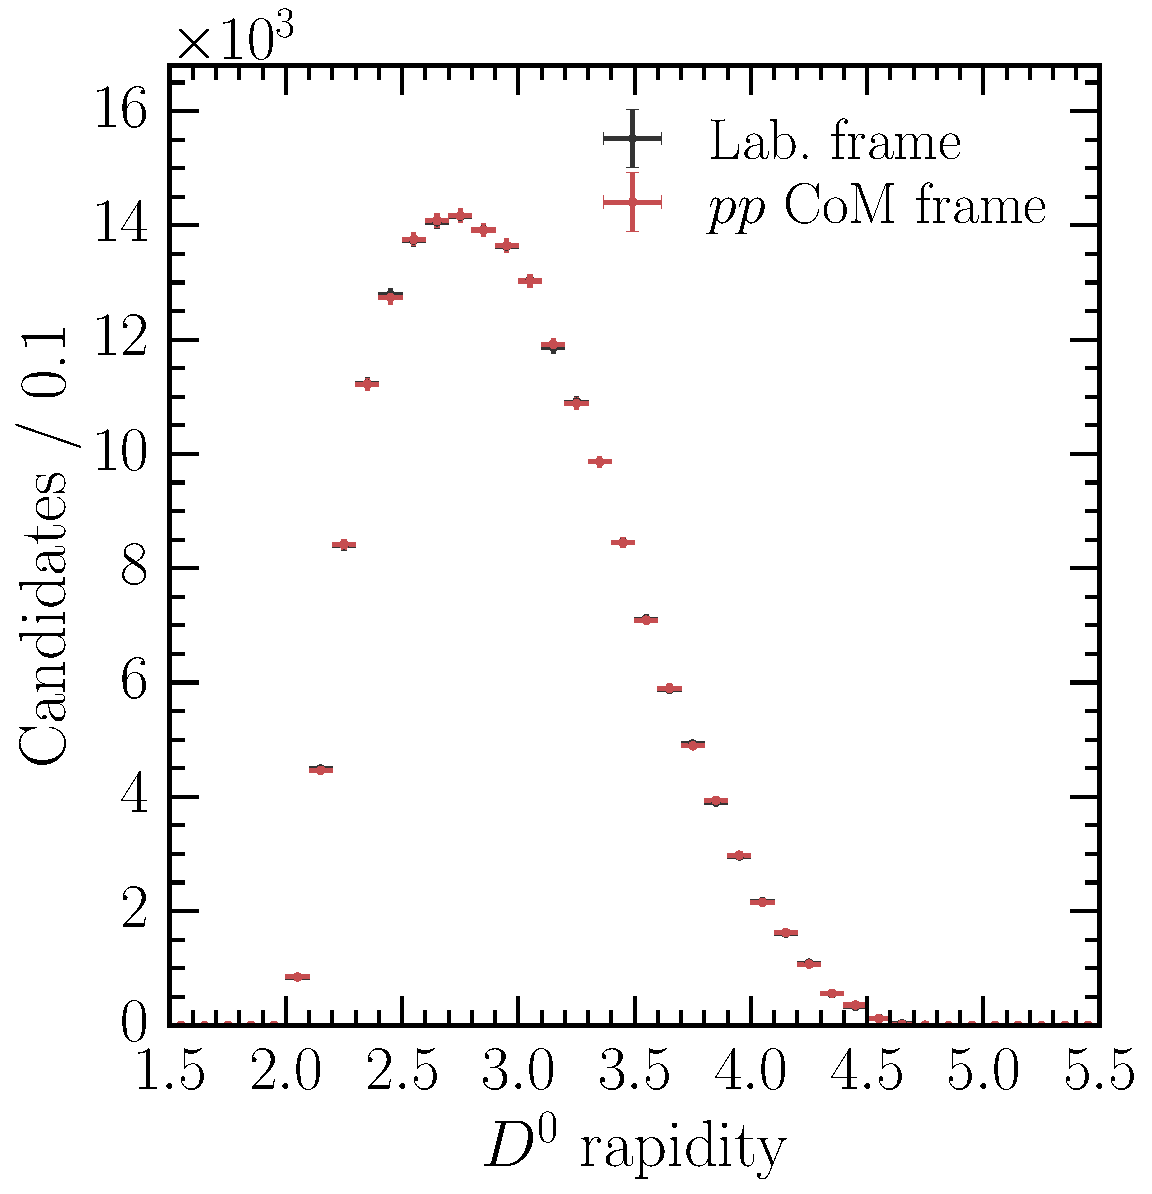
\includegraphics[width=\textwidth]{production/data/D0ToKpi_MC_Y}
    \caption{\rapidity}
    \label{fig:prod:data:com_boost:y}
  \end{subfigure}
  \caption{%
    Distributions of \PDzero\ \pT~(\subref*{fig:prod:data:com_boost:pt}) and 
    \rapidity~(\subref*{fig:prod:data:com_boost:y}) as measured in the 
    laboratory frame (black) and in the proton-proton centre-of-mass~(CoM) 
    frame (red), in the simulated \DstToDzpi, with \DzToKpi, dataset.
  }
  \label{fig:prod:data:com_boost}
\end{figure}
